\documentclass[11pt]{article}
\usepackage{page_style}

% %%%%%%%%%%%%%%%%%%%%%%%%%   COMMANDS   %%%%%%%%%%%%%%%%%%%%%%%%%%%%%%%%%
\newcommand{\ts}{\textsuperscript}
\newcommand{\maxnodes}{N_{nodes-max}}
\newcommand{\dth}{D_{threshold}}


% %%%%%%%%%%%%%%%%%%%%%%%%%   HEADER   %%%%%%%%%%%%%%%%%%%%%%%%%%%%%%%%%
\title{
    \huge Project Report \\ 
    Mining Data Records in Python \\ 
    \medskip
    \large Data Wrangling with Pierre Senellart \& Leonid Libkin  \\
    Master IASD - PSL University
}

\author{
    João Paulo Casagrande Bertoldo \\
    \href{mailto:joaopcbertoldo@gmail.com}{\texttt{joaopcbertoldo@gmail.com}} 
}
    
\date{April 2020}


% %%%%%%%%%%%%%%%%%%%%%%%%%   DOCUMENT   %%%%%%%%%%%%%%%%%%%%%%%%%%%%%%%%%

\begin{document}

% elements to mention
% - api 
% - extension
% - file management

% setup.py not been tested


% https://github.com/joaopcbertoldo/pymdr

% %%%%%%%%%%%%%%%%%%%%%%%%%   ABSTRACT   %%%%%%%%%%%%%%%%%%%%%%%%%%%%%%%%%
{
    \setstretch{.7} 
    \maketitle

    \begin{abstract}
    
    This project is part of the evaluation of the course \href{https://moodle.di.ens.fr/enrol/index.php?id=14}{\textit{Data Wrangling}} with Professors Pierre Senellart and Leonid Libkin as part of the \href{https://www.lamsade.dauphine.fr/wp/iasd/en/}{Master's degree IASD} at the \href{https://www.psl.eu/en}{PSL University} (session 2019/2020).
    \medskip
    
    This report presents a review on my implementation of the algorithm described by \cite{mdr} in the paper \say{Mining Data Records in Web Pages}. 

    \end{abstract}
}

\tableofcontents
\newpage

% %%%%%%%%%%%%%%%%%%%%%%%%%   BODY   %%%%%%%%%%%%%%%%%%%%%%%%%%%%%%%%%

\section{Introduction}


\section{Original Paper}

To implement this algorithm, I based myself on \cite{mdr-technical}. It was published in 2003 and, according to Semantic Scholar \citep{mdr-semantic-scholar}, this article has been cited over 400 times, of which more than 90 articles were highly influenced by it.

\subsection{Authors}

\paragraph{Bing Liu}

Liu is a Distinguished Professor of Computer Science at the University of Illinois at Chicago (UIC). He is the author of the book \emph{Web Data Mining} \citep{web-data-mining}. His main areas of interest are data mining and machine learning. He published many articles, like the one used for this project, about data mining applied to data from the web. More recently, Liu has worked and written about sentiment analysis - having published two books on the subject \citep{liu-page}.

\paragraph{Robert L. Grossman}

Robert was a professor at the university of Illinois at Chicago for over more the 20 years. Nowadays he is a professor in several departments at the University of Chicago. Grossman has received several awards and makes part of a number of advisory boards. He is, for instance, Chair of the Open Commons Consortium (OCC). Moreover, he is also an ACM Fellow since 2016 \citep{robert-page, robert-linkedin}.

\paragraph{Yanhong Zhai}

Yanhong was, by the time of the publication, a PhD student at the University of Illinois at Chicago. Since she received her PhD degree in 2006, Yanhong has been working in Microsoft. Having worked as Software Development Engineer (SDE) for more than 10 years, notably in web data mining and business inference, she is now a Principal SDE in the company \citep{yanhong-page, yanhong-linkedin}.

\subsection{Overview}

The article reports about the algorithm so called \say{Mining Data Records} (MDR). A \emph{data record} is a structured object on a page that holds information about some entity. The latter is supposedly from some database of records that is exposed via the website. For instance, a data record can be a product on a market place website like Amazon (Figure \ref{fig:pianos}).

\begin{figure}
  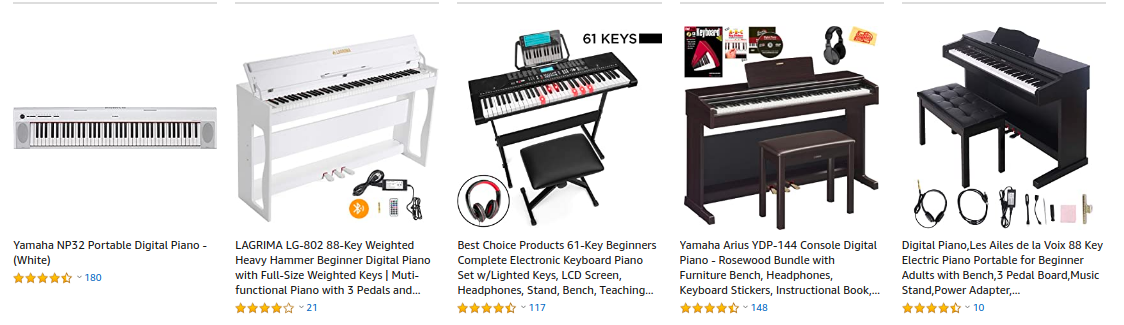
\includegraphics[width=\linewidth]{fig/pianos.png}
  \caption{Sample page from \href{www.amazon.com}{www.amazon.com} with data records about pianos. Each product offered on the page is a data record - that is, an object containing an image, a title, a rating, and the number of purchases of the product.}
  \label{fig:pianos}
\end{figure}

MDR finds data records inside table tags in HTML pages without using any heuristics about the page's contents or topic. Here bellow, I briefly describe the article's contents, but the reader is encouraged to read the short \citep{mdr} or technical \citep{mdr-technical} version of the original publication for more details.


\paragraph{Rationale}

The core of the algorithm is based on three ideas: the notion of Generalized Node (GNode for short), Data Region (DR), and a measure of distance between GNodes. A GNode is a set of $n \in {1, ..., \maxnodes}$ HTML adjacent nodes (thus, nodes under the same parent node)\footnote{The HTML structure is considered to be a tree structure where tags inside another are children of the latter.}. A DR is a set of adjacent GNodes that are \emph{similar}, where \say{similar} means that the distance between each 2 directly adjacent GNodes is bellow the threshold $\dth$. The measure of distance is the Normalized Levenshtein Edit Distance \footnote{See the \cite{lev-dist-wiki} for more information.}:

\begin{equation}\label{eq:dist}
    d\left(s_{1}, s_{2}\right)=\frac{LevenshteinEditDist\left(s_{1}, s_{2}\right)}{\frac{\text {length}\left(s_{1}\right)+\text {length}\left(s_{2}\right)}{2}} \in [0, 1]
\end{equation}

The values of $\maxnodes$ and $\dth$ are parameters of the algorithm and the authors reported using, respectively, $10$ and $0.30$. Once the DRs are found in the HTML node tree, there is a last scan over them that figure out which ones are data records or not.

% todo: schematic here?


\paragraph{Experimental results}

The authors tested MDR on $46$ different pages, with a total of $621$ objects (data records). They reported a precision and a recall of, respectively, $100\%$ and $99.8\%$, outperforming (by far) other algorithms previously proposed by other authors. The list of websites used by them can be seen on the Table 1 in \cite{mdr}. 


\paragraph{Issues}

Unfortunately, the authors did not make available any reference implementation. They also did not make public the specific cached HTML pages that they used to test the algorithm on, or even the specific pages used (only the websites). Some of the websites mentioned in the their test set do not exist anymore (like \href{http://www.bookbuyer.com}{\textit{bookbuyer.com}} and \href{http://www.codysbooks.com}{\textit{codysbooks.com}}) or became a completely different website (such as \href{https://www.eveonline.com/}{\textit{eveonline.com}}). Moreover, they do not describe how the data was labeled or inspected, making it harder to reproduce their precision and recall metrics.

\section{Implementation}

% implementation + viz...
% core, utils, api
\paragraph{Code structure}

\subsection{Core}

\paragraph{Dependencies}
% lxml
% levenshtein library
% - lxml choice
% - graphviz choice --> conversion with lxml

\paragraph{Classes}
% -- gnode
% -- gnode pair
% -- data region 
% -- data record 
% -- MDREditDistanceThresholds --> varying thresholds, mistake, but why it made sense
% -- WithBasicFormat --> quick comment

\paragraph{Functions}
% -- only_1b1 inside _compare_combinations
% -- find_data_records --> not specifically given, just described in the text

\paragraph{Parameters}

\paragraph{Node naming}

% -- node namer == utility, should've done differently?, bug?, simpler with fun? --> a bit more of arguments carrying, it was necessary bc (reason?) the HtmlElements do not have constant id/hash, maybe it's the same problem as with the str???, would have chosen another framework if I knew...


\paragraph{Intermediate structures}

\subsection{Web API and Chrome Extension}

\paragraph{Files management}

\subsection{Unit tests}

\section{First results}

% slowliness due to considering all the tags

% !! in technical report, page 2, col left, section 1 (intro)
%   "It currently
% finds all data records formed by table and form related tags, i.e.,
% table, form, tr, td


\section{Algorithm tuning}

\subsection{Investigation}

\paragraph{Factors and hypothesis}
% - table elements only --> cutting off for performance in computing distances
% - table elements only --> too little results
% -- manual check that there are not many tables
% -- later confirmed in the results viz

\paragraph{Threshold}

\paragraph{HTML Lists}

\paragraph{Edit distance distortion issue}

\subsection{Experiments}

\paragraph{Test pages}

% - cached pages not available --> certainly aged up
% - pages that do not exist anymore --> had to verify myself
% - did not give exact urls --> i picked some random ones


% OMNI project page pointed out in the project is not available anymore
% http://disl.cc.gatech.edu/Omini/
% paper:
%     A Fully Automated Object Extraction System for the World Wide Web
%     https://ieeexplore.ieee.org/document/918966?arnumber=918966
%     https://www.researchgate.net/publication/3895240_A_Fully_Automated_Object_Extraction_System_for_the_World_Wide_Web

% ... apparently it move to here: https://www.cc.gatech.edu/projects/disl/Omini/
%     pages are cached locally...
%         https://www.cc.gatech.edu/projects/disl/Omini/local.html
%         cannot access

% neither is the IEPAD one
% http://140.115.155.99

% so, i collected my own pages...

\paragraph{Files management}

\paragraph{Pre & Post-Processing}

\paragraph{Python string hashing issue}
% -- str hash problem...

\subsection{Results}
% - table elements only --> cutting of for performance in computing distances

\paragraph{Evaluation}

- no precise description of tagging/labelling --> how to measure precision/recall? --> simplified way of counting to investigate --> coloring the background for visual inspection

\paragraph{Reproduction}

% nb with comments
% evaluating_stuff-with-list-with-cleanup.ipynb


% %%%%%%%%%%%%%%%%%%%%%%%%%   REFS   %%%%%%%%%%%%%%%%%%%%%%%%%%%%%%%%%
\newpage
\bibliography{refs} 


\end{document}